\section{Versuchsaufbau}
\label{sec:Versuchsaufbau}
Als Grundlage des Aufbaus dient eine optische schiene. Das Gasentladungsrohr sowie ein Justierlaser zur Kontrolle der Ausrichtung der optischen Elemente entlang der optischen Achse sind bereits montiert und vorjustiert.
\autoref{fig:aufbau_echt} zeigt den Versuchsaufbau bei laufendem HeNe-Laser.
\begin{figure}
  \centering
  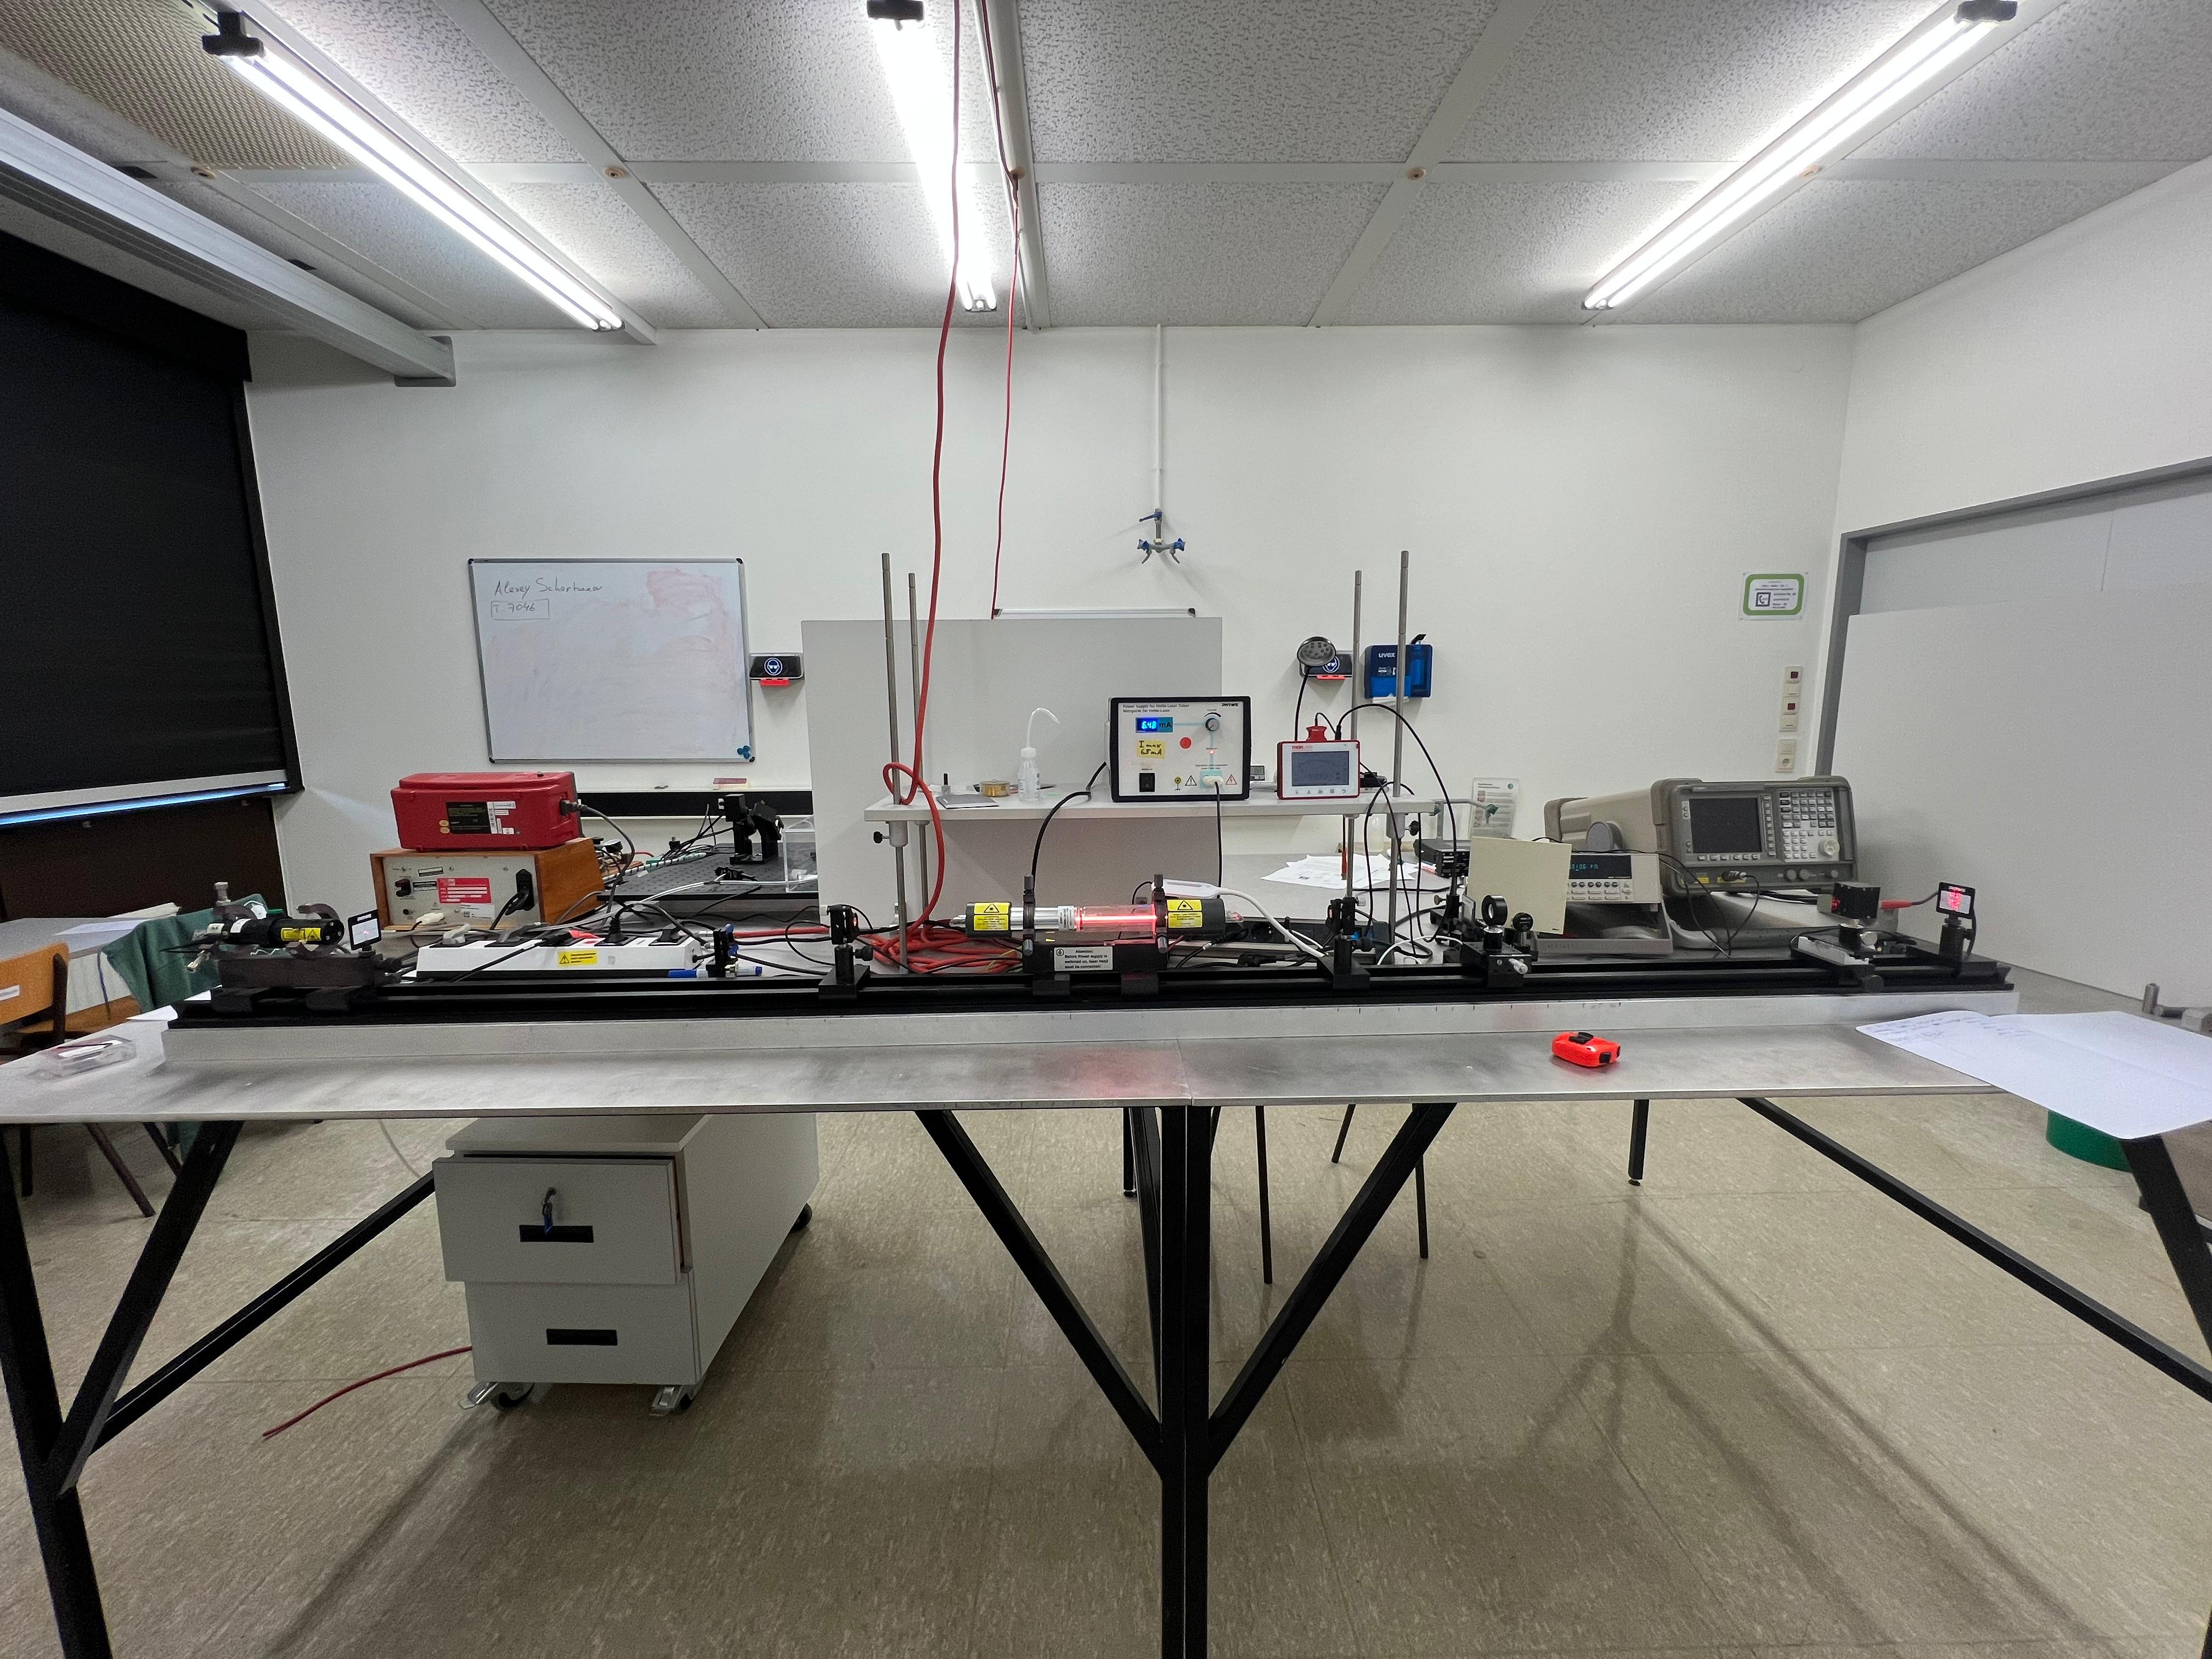
\includegraphics[width=0.7\textwidth]{content/images/lasertisch.jpeg}
  \caption{Aktivierter HeNe-Laser auf der für den Versuch verwendeten optischen Schiene.}
  \label{fig:aufbau_echt}
\end{figure}
\FloatBarrier\noindent
Die weiteren für den Versuch benötigten optischen Elemente sind zwei Lochblenden mit Fadenkreuz zur Justierung, zwei Photodioden, eine Streulinse zur Vergrößerung des Laserstrahls, mehrere optische Gitter und ein Wolframdraht mit $d = 5\,\unit{\micro\meter}$ Durchmesser.
In \autoref{fig:spiegel} sind die Eigenschaften der verwendeten Resonatorspiegel aufgelistet.
\begin{figure}
  \centering
  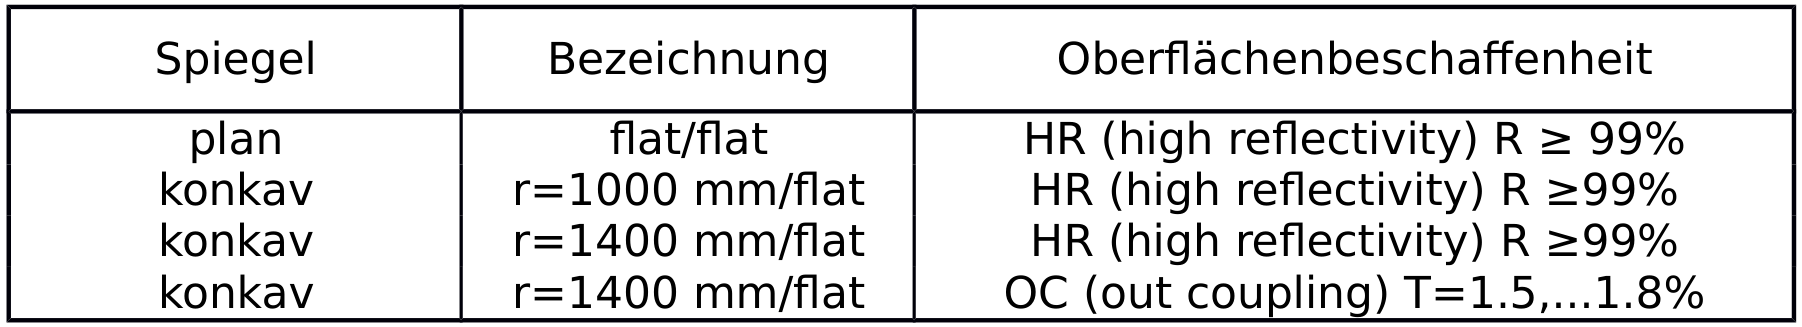
\includegraphics[width=0.7\textwidth]{content/images/spiegel.png}
  \caption{Eigenschaften der verwendeten Resonatorspiegel~\cite[3]{V61}.}
  \label{fig:spiegel}
\end{figure} 
\FloatBarrier\noindent
Für den Versuch werden die Spiegel aus der ersten, dritten und vierten Zeile verwendet.
\section{Durchführung}
\label{Durchführung}
Zuerst wird die Justierung des Aufbaus überprüft. Dazu wird zunächst die Gasentladungsröhre entlang des Justierlasers positioniert.
Danach wird der auskoppelnde Spiegel in den Strahlengang eingebracht und so eingestellt, dass die Beugungsringe des Justierlasers mittig auf Fadenkreuz der Lochblende sind.
Der zweite Resonatorspiegel wird ebenso justiert und anschließend die Gasentladungsröhre eingeschaltet. 
Der zweite Resonatorspiegel wird so lange nachjustiert, bis die Laseraktivität einsetzt.
\subsection{Messung der Stabilitätsbedingung}
  Für die Überprüfung der Stabilitätsbedingung werden die Resonatorspiegel auf maximale Laserintensität justiert. 
  Anschließend wird die Resonatorlänge vergrößert, bis die maximale stabile Resonatorlänge erreicht ist, oder keine Laseraktivität mehr erreicht werden kann. 
  Dazu wird die Spiegelausrichtung so nachjustiert, dass das Intensitätsmaximum beibehalten wird.\\
  Dies wird zuerst für die beiden konkaven Spiegel durchgeführt. 
  Danach wird der zweite Resonatorspiegel durch den flachen Spiegel ersetzt und die Messung wiederholt.
\subsection{Messung der Moden $\mathrm{TEM}_{00}$ und $\mathrm{TEM}_{01}$}
Für die Messung der transversalen Moden muss der Laserstrahl vergrößert werden. Dazu wird die Streulinse in den Strahlengang ausserhalb des Resonators eingebracht und eine Photodiode montiert.
Die Photodiode sitzt auf einer senkrecht zur optsichen Achse verschiebbaren Schiene mit einer Millimeter-Skala und $1/10$ Nonius.\\
